\chapter{力学性能实验与组织表征}

\section{TC4钛合金的力学实验过程}
力学性能是表征材料性能的重要参数,本实验采用常规的拉伸试验来测量式样的力学性能。测量的包括屈服强度、抗拉强度。

采用拉伸试验机对经固溶时效热处理工艺的试样进行常温微拉伸性能测试,拉 伸速率为2mm/min,每组热处理工艺进行三次测定,取其平均值,微拉伸试样尺寸

在某型号万能力学试验机上测试得到的结果如下:

\begin{table}[htbp]
	\centering
	\caption{\ti 合金的力学性能实验结果}
	\label{sec:mystrength}
		\begin{tabular}{ccc}
			\toprule
			实验编号&$ R_m $/Mpa&$ R_{p0.2} $/Mpa \\
			\midrule
			1 & 950 & 866\\
			2 & 946 & 872\\
			3 & 976 & 884\\
			4 & 988 & 894\\
			5 & 990 & 920\\
			6 & 972 & 886\\
			7 & 966 & 820\\
			8 & 978 & 849\\
			9 & 959 & 836\\
			\bottomrule
		\end{tabular}
\end{table}
\newpage
\section{TC4钛合金的显微组织表征}
试验期间用来观察组织和分析相结构的检测方法,主要包括光学显微镜 (OM)、扫描式电子显微镜 (SEM)、X射线衍射分析 (XRD)以及透射式电子显微镜 (TEM)等。

将固溶与时效后的试件进行线切割截取显微组织分析试样,截取后的试样进行 150\#、400\#、1000\#、1500\#、2000\#、2500\#金相砂纸磨制,对磨制后的试样采用 0.05umSiO2抛光液在抛光机上进行抛光,去除试样表面的划痕或杂质颗粒,经抛光后的试样采用$ HF:HNO3:H2O=2:4:94 $的Kroll试剂进行腐蚀。腐蚀后的试样分别采用光 学显微镜(OM)、扫描电子显微镜(SEM)对其微观形貌进行观察。


三种不同固溶温度得到的试样组织如下:
\begin{figure}[h!]
	\centering
	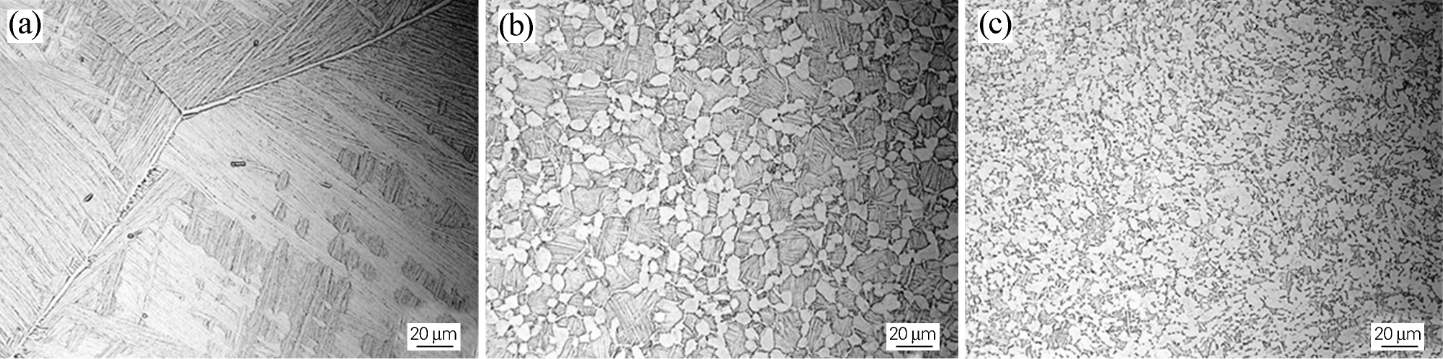
\includegraphics[width=0.7\linewidth]{pic/demo-mico}
	\caption{不同热处理工艺下 TC4 钛合金的显微组织}
	\label{fig:demo-mico}
\end{figure}